% ============================================================
% Methodology, Results, and Discussion
% Research Leadership in International Collaborations Involving
% Ghanaian Researchers in Biomedical Science and Engineering
% ============================================================
\documentclass[12pt, a4paper]{article}

% ── Packages ──
\usepackage[utf8]{inputenc}
\usepackage[T1]{fontenc}
\usepackage{lmodern}
\usepackage[margin=2.5cm]{geometry}
\usepackage{amsmath, amssymb}
\usepackage{booktabs}
\usepackage{multirow}
\usepackage{graphicx}
\usepackage{float}
\usepackage{longtable}
\usepackage{array}
\usepackage{caption}
\usepackage{subcaption}
\usepackage[hidelinks]{hyperref}
\usepackage{setspace}
\usepackage{rotating}
\usepackage{pdflscape}
\usepackage{xcolor}
\usepackage{natbib}

\onehalfspacing
\graphicspath{{./}}

\begin{document}

% ============================================================
\section{Methodology}
% ============================================================

\subsection{Data Source and Study Design}

This cross-sectional bibliometric study analysed international collaborative publications involving Ghanaian researchers in biomedical science and engineering between 2000 and 2025. Publication metadata were retrieved from OpenAlex, an open-access scholarly database indexing over 250 million works with structured affiliation, authorship, and citation data. OpenAlex provides granular author-level information---including institutional affiliations, authorship order, and corresponding author flags---that is essential for affiliation-based leadership analysis.

The initial dataset comprised 46,945 publications tagged to Ghanaian institutions across biomedical and engineering fields. Three sequential inclusion criteria were applied: (1)~publication year between 2000 and 2025 ($n = 41{,}788$); (2)~international collaboration, defined as at least one co-author affiliated with a non-Ghanaian institution ($n = 25{,}949$); and (3)~at least two authors per publication ($n = 24{,}768$). The final study set of 24,768 works contained 223,453 authorship records representing 93,203 unique authors across 203 countries.

\begin{figure}[H]
\centering
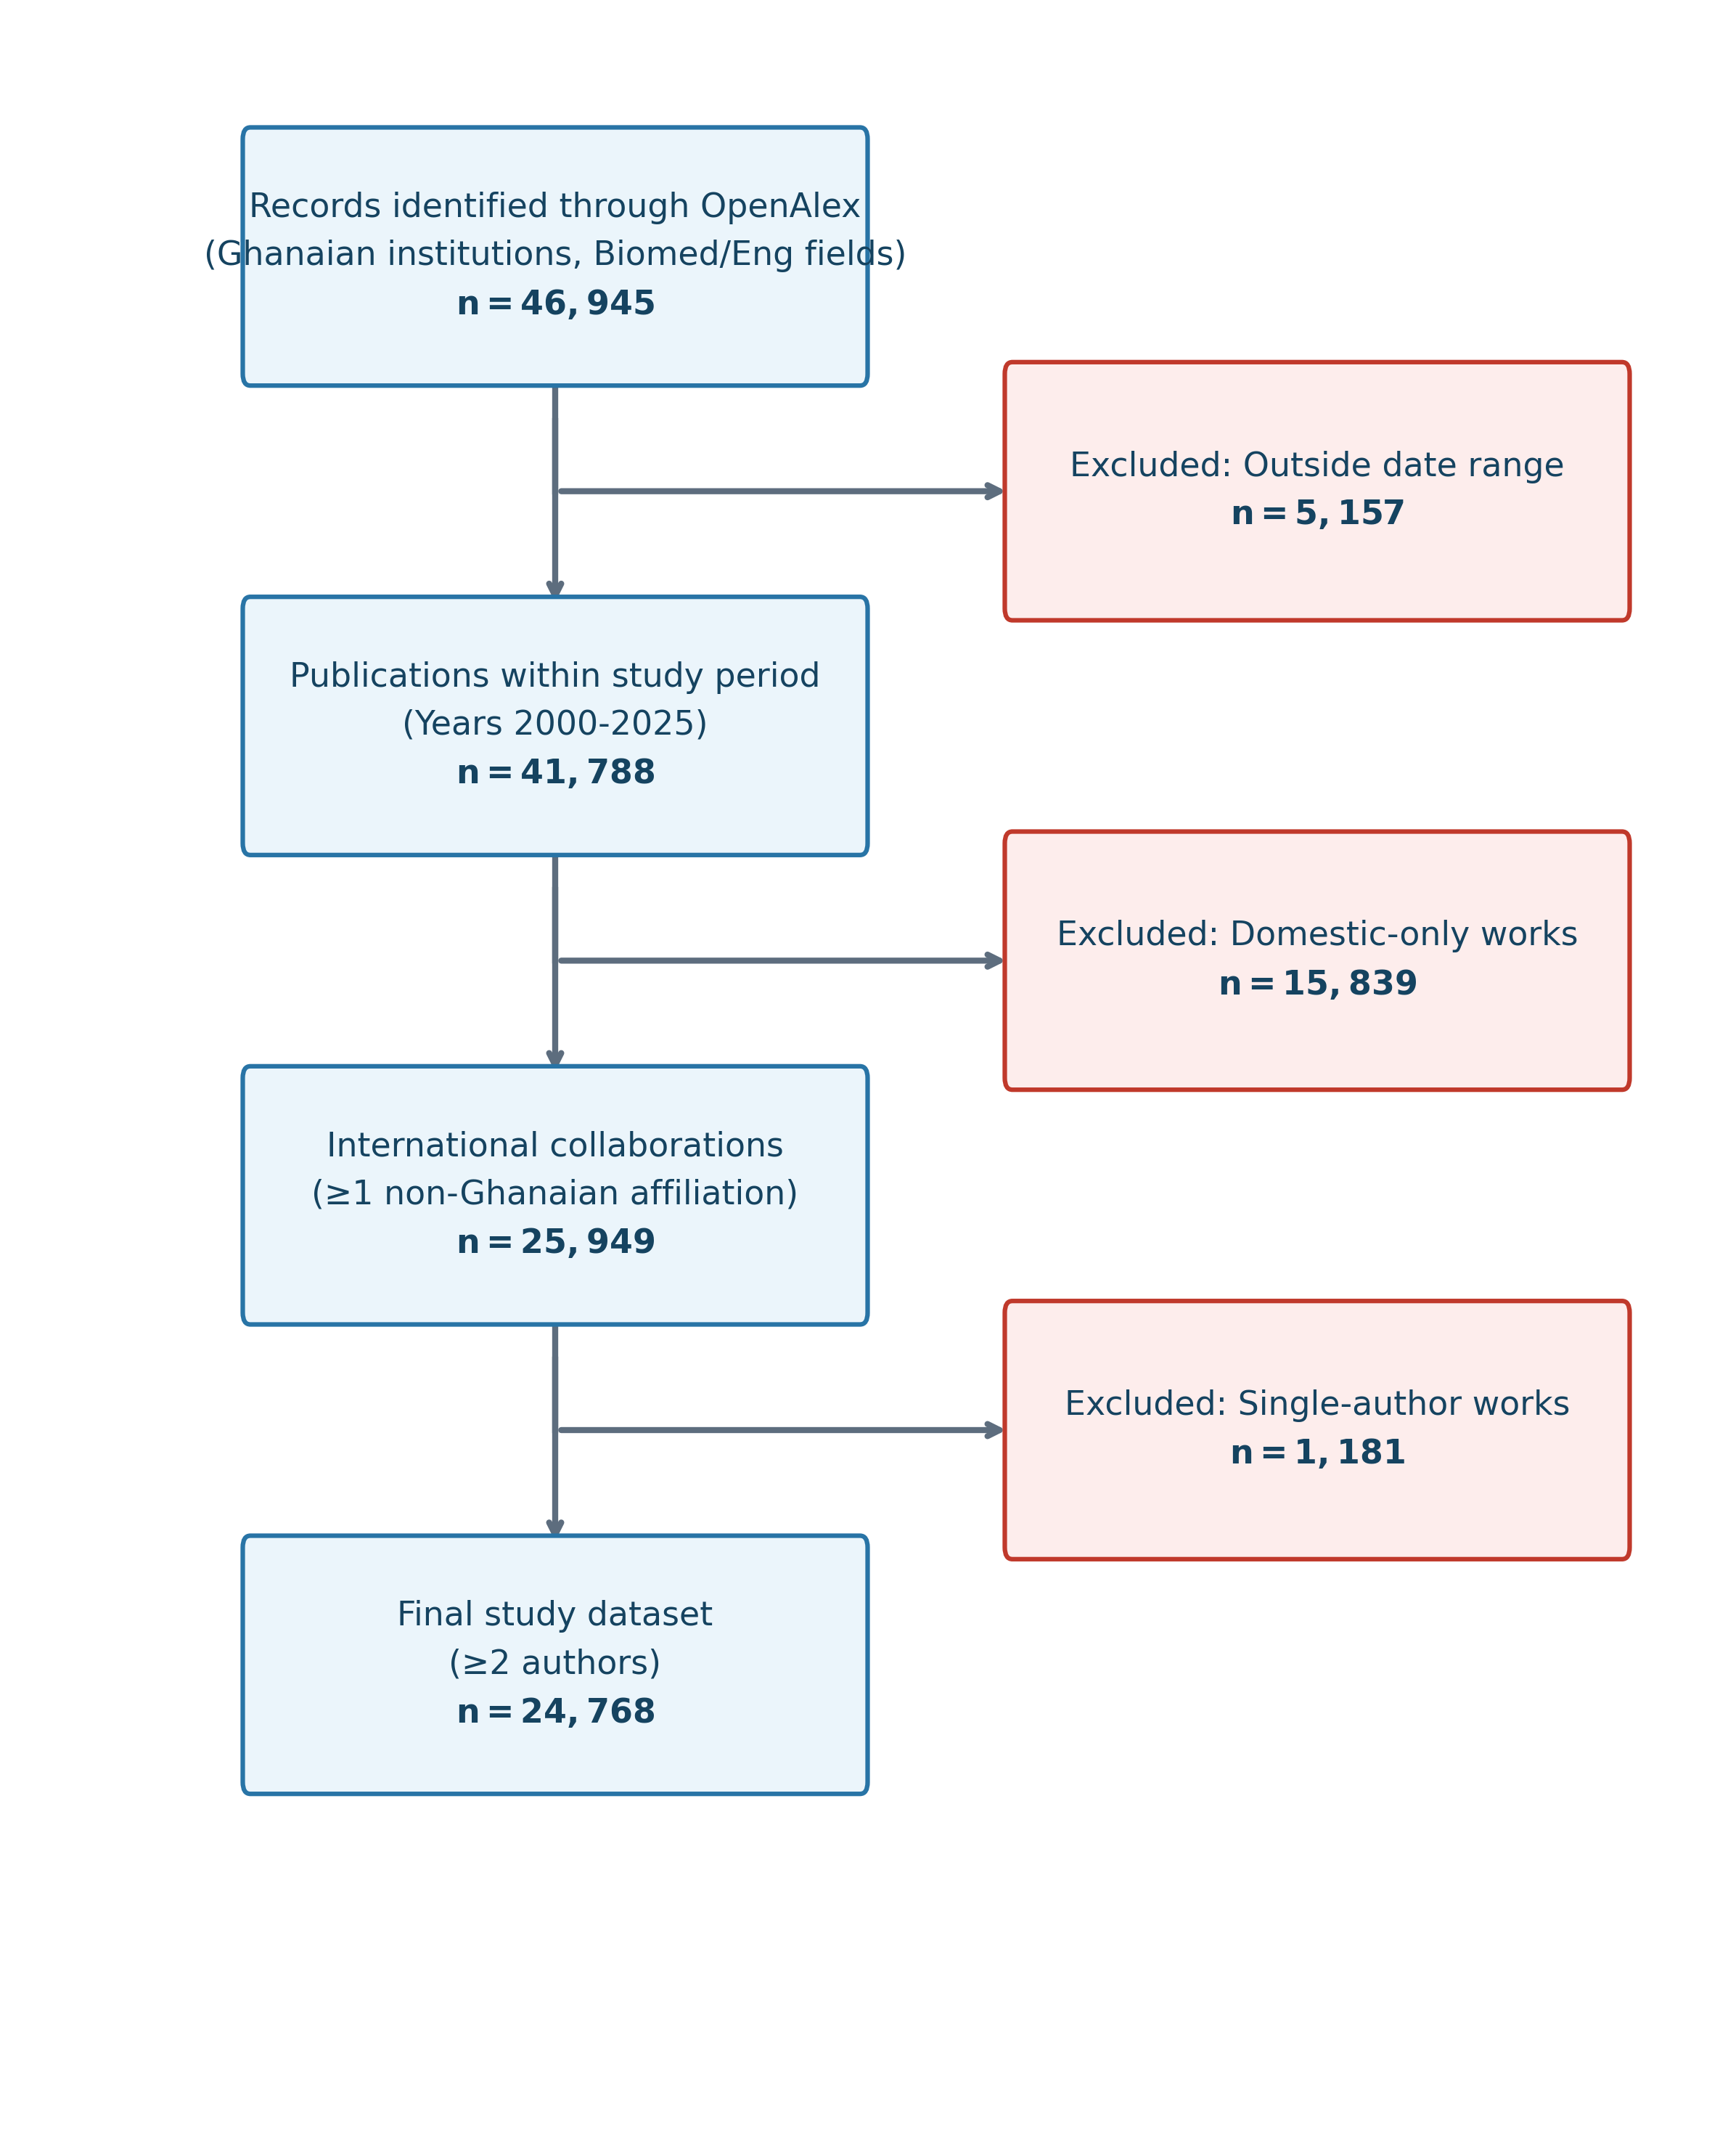
\includegraphics[width=0.85\textwidth]{chart_00_prisma_flow.png}
\caption{PRISMA-style flow diagram detailing the application of inclusion and exclusion criteria to arrive at the final study dataset of 24,768 international collaborative publications.}
\label{fig:prisma}
\end{figure}

\subsection{Outcome Variables: Research Leadership}

Research leadership was operationalised through three authorship positions, each carrying a distinct signal in biomedical publishing conventions. \emph{First authorship} denotes the researcher who performed the most substantive analytical work and led the manuscript writing. \emph{Last authorship} signals senior intellectual leadership---typically the principal investigator or laboratory director who conceived the study. \emph{Corresponding authorship} designates the researcher who manages the manuscript through peer review, handles editorial correspondence, and serves as the long-term contact for the work.

For each work in the study set, the author occupying each of these three positions was identified and classified into one of three affiliation categories: \emph{Ghanaian} (affiliated exclusively with Ghanaian institutions), \emph{Dual-affiliated} (holding affiliations in both Ghana and at least one other country), or \emph{Non-Ghanaian} (affiliated exclusively with non-Ghanaian institutions). An important definitional note: ``Ghanaian'' is determined by institutional affiliation, not nationality. A British researcher employed at the University of Ghana is classified as ``Ghanaian''; a Ghanaian national at Harvard with no current Ghanaian affiliation is classified as ``Non-Ghanaian.'' This classification likely biases toward higher reported Ghanaian leadership, as some researchers categorised as ``Ghanaian'' may be expatriate investigators.

Corresponding author data were available for 99.9\% of works ($n = 24{,}752$). However, validation revealed that in 80.1\% of works, the first author was also flagged as the corresponding author---a rate substantially higher than the 50--60\% typical in biomedical publishing, suggesting that OpenAlex may impute first authors as corresponding when explicit metadata is unavailable. This partial collapse of corresponding into first authorship is noted as a caveat throughout. We retain the corresponding author analysis because the results show meaningfully different patterns from first authorship (e.g., a steeper temporal decline, a larger funding $\chi^2$), suggesting the measure captures distinct signal despite imputation.

\subsection{Predictor Variables}

Seven predictor variables were constructed for each publication:

\begin{enumerate}
    \item \textbf{Partner bloc}: Non-Ghanaian co-authors were classified by geographic region, and each work was assigned to one of eight categories: Western ($n = 10{,}836$; 43.8\%), Multi-bloc ($n = 8{,}691$; 35.1\%), African ($n = 2{,}671$; 10.8\%), East Asian ($n = 1{,}788$; 7.2\%), South Asian ($n = 441$; 1.8\%), MENA ($n = 222$; 0.9\%), Other ($n = 73$; 0.3\%), and Latin American ($n = 46$; 0.2\%). Works with partners spanning multiple blocs were classified as ``Multi-bloc.''
    
    \item \textbf{Team size}: Total number of authors per work (median = 6, IQR: 4--10).
    
    \item \textbf{Country count}: Number of distinct countries represented among co-authors (median = 2, IQR: 2--3).
    
    \item \textbf{Funding status}: Binary indicator of whether the work acknowledged external funding, derived from OpenAlex funding records (28,541 records linked to the study set).
    
    \item \textbf{COVID era}: Binary indicator (0 = 2000--2019; 1 = 2020--2025).
    
    \item \textbf{Open access status}: Binary indicator from OpenAlex metadata.
    
    \item \textbf{Disciplinary field}: Top-level OpenAlex concept classification, grouped into Health Sciences (69.4\%), Physical Sciences (16.6\%), Life Sciences (14.0\%), and subfields including Engineering, Medicine, Nursing, and Health Professions.
\end{enumerate}

\subsection{Statistical Analysis}

\subsubsection{Descriptive and Bivariate Analyses}

Proportions and 95\% Wilson confidence intervals were computed for Ghanaian, dual-affiliated, and non-Ghanaian leadership at each authorship position. Chi-square goodness-of-fit tests assessed whether the distribution of affiliation categories in leadership positions deviated from the overall authorship composition. Chi-square tests of independence compared leadership rates across partner blocs, funding categories (Northern-funded, Ghanaian-funded, unfunded), and COVID era (pre- vs.\ post-2020), with Bonferroni correction applied to pairwise comparisons ($\alpha = 0.0167$ for three comparisons).

Citation impact was assessed using Field-Weighted Citation Impact (FWCI; available for 91.6\% of works). Mann-Whitney $U$ tests compared FWCI distributions by first author category. The proportion of works in the top 10\% of cited publications was computed within the FWCI-available subset ($n = 22{,}684$).

\subsubsection{Temporal Trend Analysis}

Three complementary approaches assessed temporal trends. \emph{Bivariate logistic regression} with publication year (centred at 2000) as the sole predictor estimated unadjusted trends. \emph{Mann-Kendall tests} assessed the presence of monotonic trends in annual leadership proportions, with Sen's slope estimating the magnitude of change in percentage points per year. \emph{Multivariate logistic regression} (described below) estimated adjusted temporal trends after controlling for structural confounders.

\subsubsection{Multivariate Logistic Regression}

Three separate logistic regression models were fit---one each for first, last, and corresponding authorship---with the binary outcome defined as Ghanaian or dual-affiliated (1) versus non-Ghanaian (0). Predictors included year (centred), COVID era, country count, author count, funding status, open access status, partner bloc (dummy-coded with African as the reference), and disciplinary field (dummy-coded with Biochemistry/Genetics as the reference). Variance Inflation Factors (VIF) were computed to assess multicollinearity; all values were $\leq 2.80$, well below the conventional threshold of 5.0. Model fit was assessed via AIC and McFadden's pseudo-$R^2$. Odds ratios (ORs) and 95\% confidence intervals were computed via profile likelihood.

\subsubsection{Sensitivity Analyses}

Six sensitivity analyses tested robustness: (1)~reclassification of dual-affiliated authors as either Ghanaian or non-Ghanaian; (2)~restriction to journal articles only ($n = 19{,}788$, 79.9\%); (3)~verification of $\geq$50\% corresponding author coverage across all study years; (4)~exclusion of works with $>$50 authors ($n = 337$); (5)~exclusion of COVID-topic papers ($n = 781$) to test whether pre-/post-2020 leadership shifts persist; and (6)~Bonferroni-corrected pairwise comparisons across partner blocs.

All analyses were conducted in Python 3.11 using \texttt{pandas}, \texttt{statsmodels}, \texttt{scipy}, and \texttt{matplotlib}. Confidence level was set at 95\% throughout.

% ============================================================
\section{Results}
% ============================================================

\subsection{Study Characteristics}

The 24,768 international collaborative works contained 223,453 authorship records from 93,203 unique authors across 203 countries, with linked data comprising 320,537 affiliation records, 69,961 topic classifications, and 28,541 funding records. The authorship pool comprised Non-Ghanaian (153,305; 68.6\%), Ghanaian (51,647; 23.1\%), and Dual-affiliated (18,501; 8.3\%) records. The pre-COVID period (2000--2019) contributed 9,675 works (39.1\%); the post-COVID period (2020--2025) contributed 15,093 (60.9\%), reflecting exponential growth in Ghanaian research output.

\subsection{Overall Leadership Proportions}

Non-Ghanaian researchers dominated all three leadership positions (Table~\ref{tab:overall}). The disparity was most acute for last authorship: non-Ghanaian researchers held 66.2\% of last author positions, compared to 55.1\% of first authorships and 59.9\% of corresponding authorships. Chi-square goodness-of-fit tests confirmed that leadership distributions deviated significantly from the overall authorship composition at all three positions (all $p < 0.001$).

\begin{table}[H]
\centering
\caption{Overall research leadership proportions in international collaborations involving Ghanaian researchers, 2000--2025 ($N = 24{,}768$)}
\label{tab:overall}
\begin{tabular}{l r@{\hspace{4pt}}c r@{\hspace{4pt}}c r@{\hspace{4pt}}c r}
\toprule
\textbf{Position} & \multicolumn{2}{c}{\textbf{Ghanaian}} & \multicolumn{2}{c}{\textbf{Dual-affiliated}} & \multicolumn{2}{c}{\textbf{Non-Ghanaian}} & \textbf{$\chi^2$ (df=2)} \\
\midrule
First author    & 25.8\% & (25.3--26.3) & 19.1\% & (18.6--19.6) & 55.1\% & (54.5--55.8) & 4{,}212.26*** \\
Last author     & 22.0\% & (21.5--22.5) & 11.8\% & (11.4--12.2) & 66.2\% & (65.6--66.8) & 407.07*** \\
Corresponding   & 24.5\% & (24.0--25.0) & 15.6\% & (15.2--16.0) & 59.9\% & (59.4--60.5) & 2{,}372.25*** \\
\bottomrule
\multicolumn{8}{l}{\footnotesize Percentages with 95\% Wilson confidence intervals. $***\,p < 0.001$. Goodness-of-fit against overall} \\
\multicolumn{8}{l}{\footnotesize authorship composition (68.6\% Non-Ghanaian, 23.1\% Ghanaian, 8.3\% Dual-affiliated).} \\
\end{tabular}
\end{table}

\begin{figure}[H]
\centering
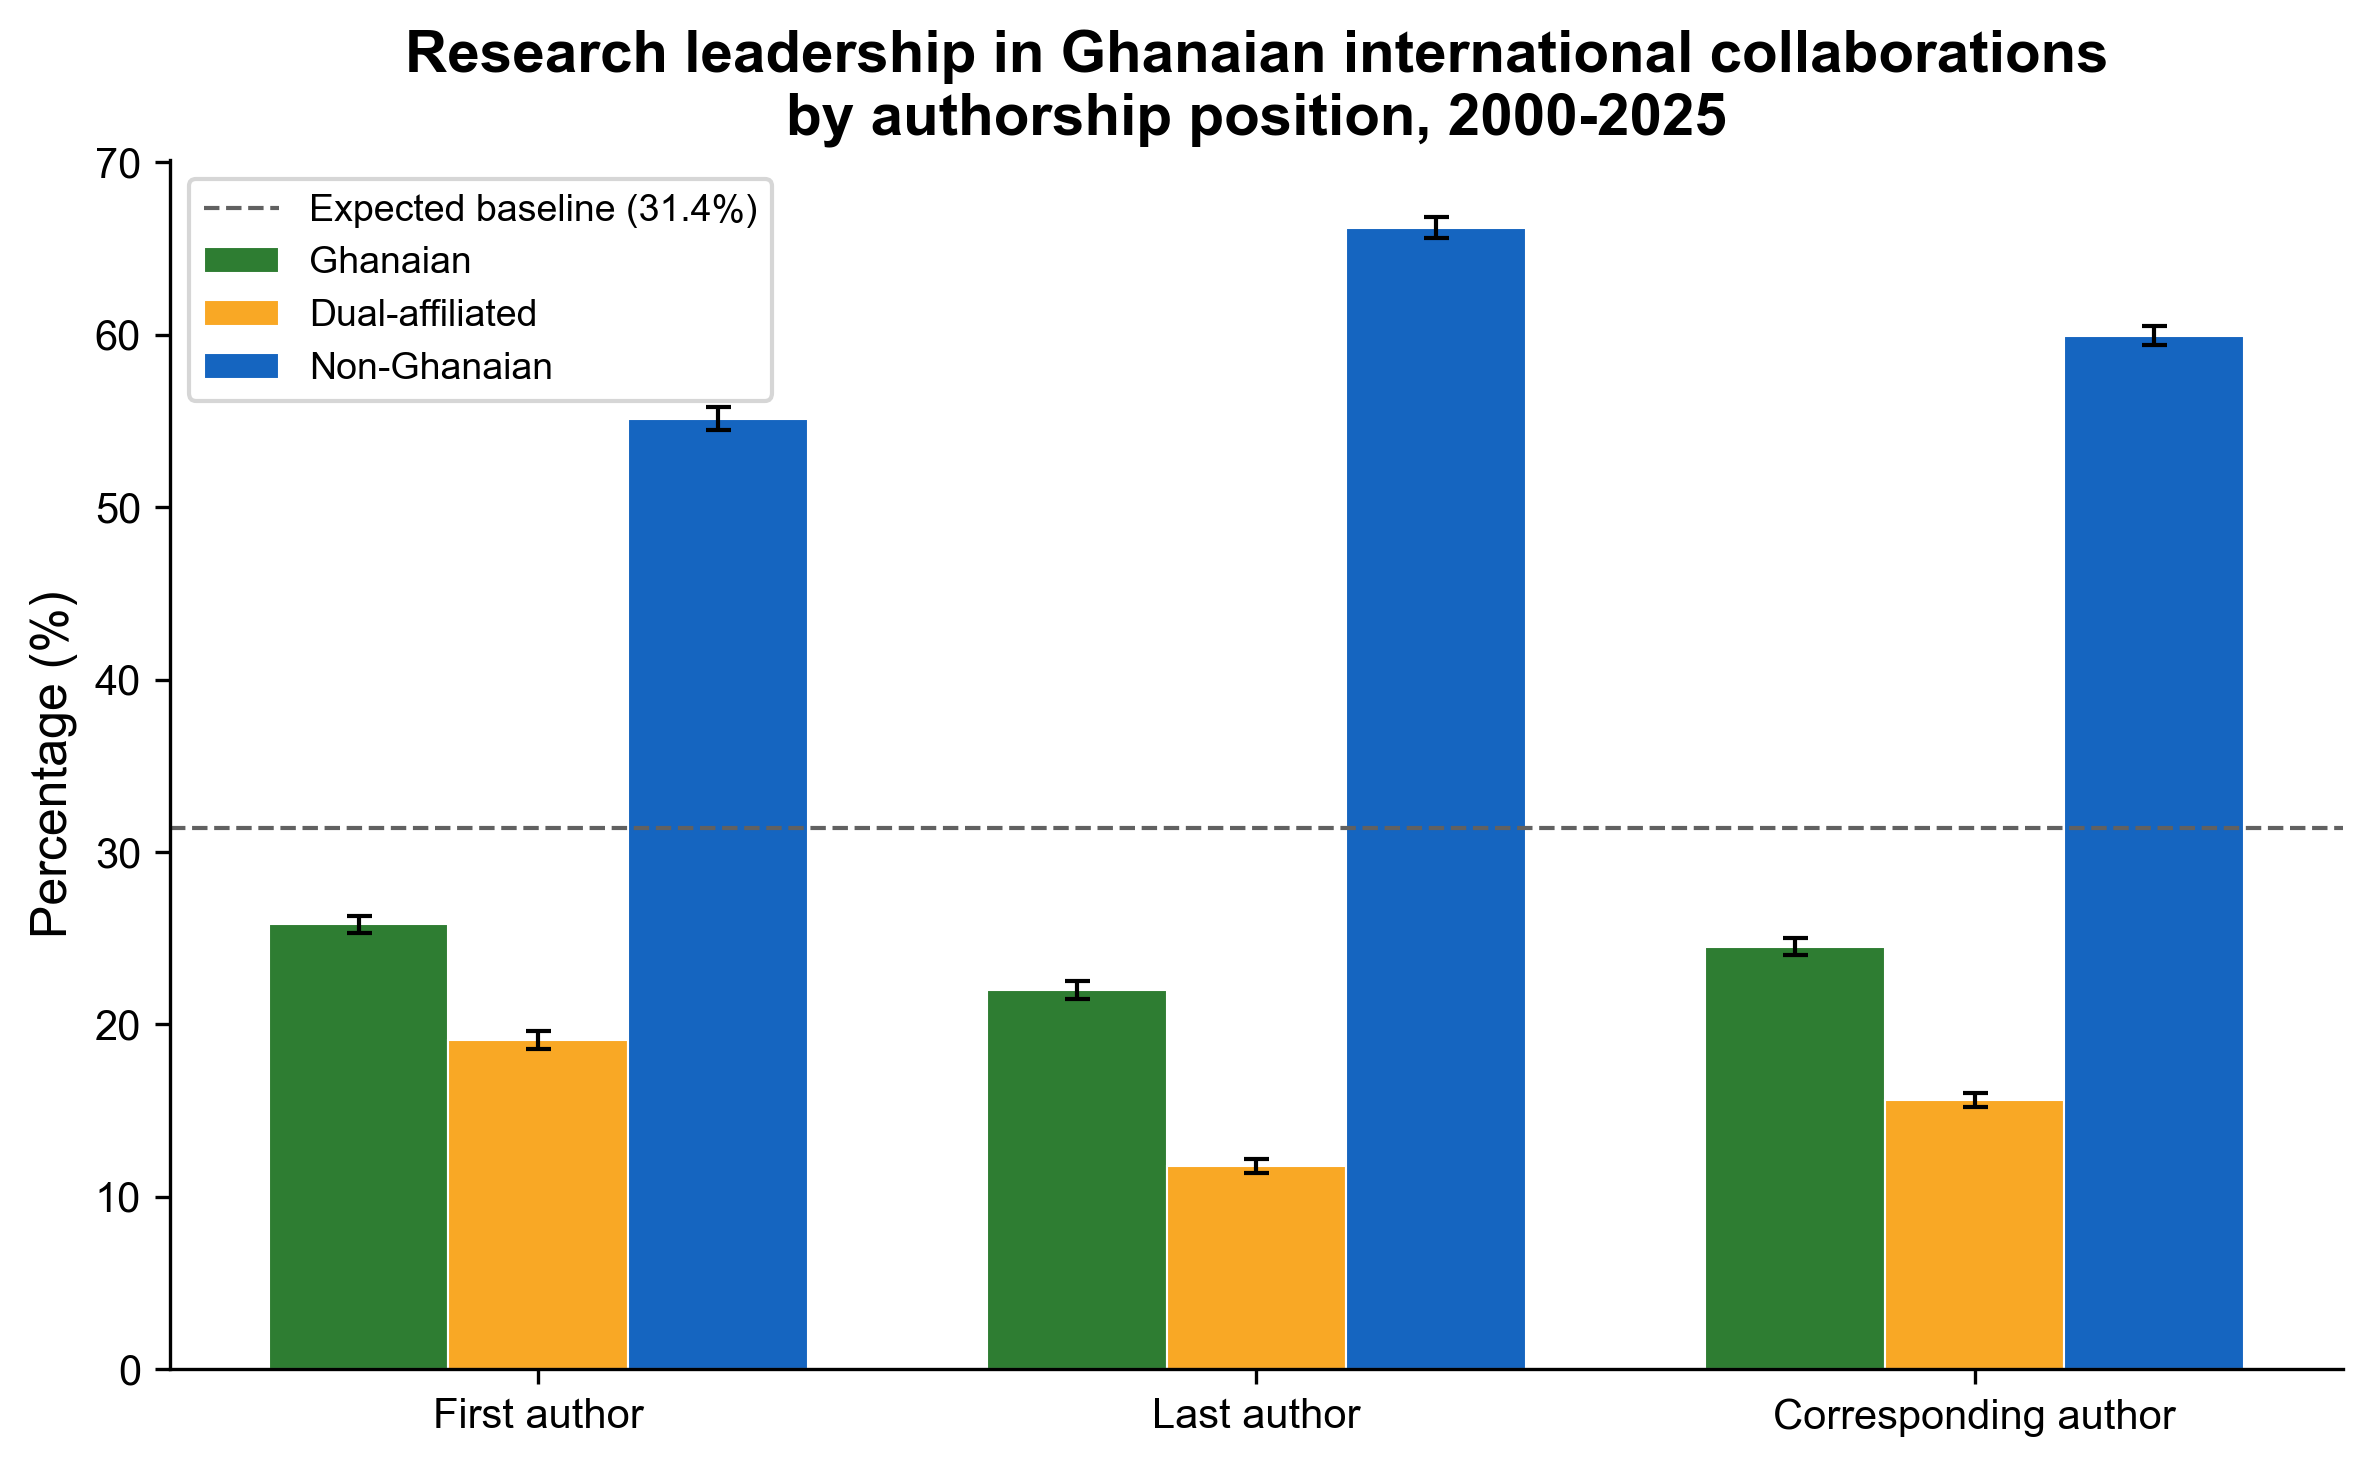
\includegraphics[width=0.88\textwidth]{chart_04_leadership_overall.png}
\caption{Overall distribution of first, last, and corresponding authorship by affiliation category ($N = 24{,}768$). Non-Ghanaian researchers dominate all three positions, with the disparity most acute for last authorship (66.2\%).}
\label{fig:overall}
\end{figure}

\subsection{Temporal Trends: A Simpson's Paradox}

Bivariate logistic regression revealed no improvement over time. First authorship showed a small but significant decline (OR = 0.994, 95\% CI: 0.990--0.999, $p = 0.008$), and corresponding authorship showed a steeper decline (OR = 0.993, 95\% CI: 0.989--0.997, $p < 0.001$). Last authorship was stable (OR = 1.001, $p = 0.685$). Mann-Kendall tests corroborated these findings: only corresponding authorship showed a statistically significant monotonic decline ($\tau = -0.320$, $p = 0.023$, Sen's slope $= -0.15$~pp/year). Figure~\ref{fig:trends} illustrates the temporal trajectory for first authorship, showing the declining aggregate proportion alongside rising publication volume.

\begin{figure}[H]
\centering
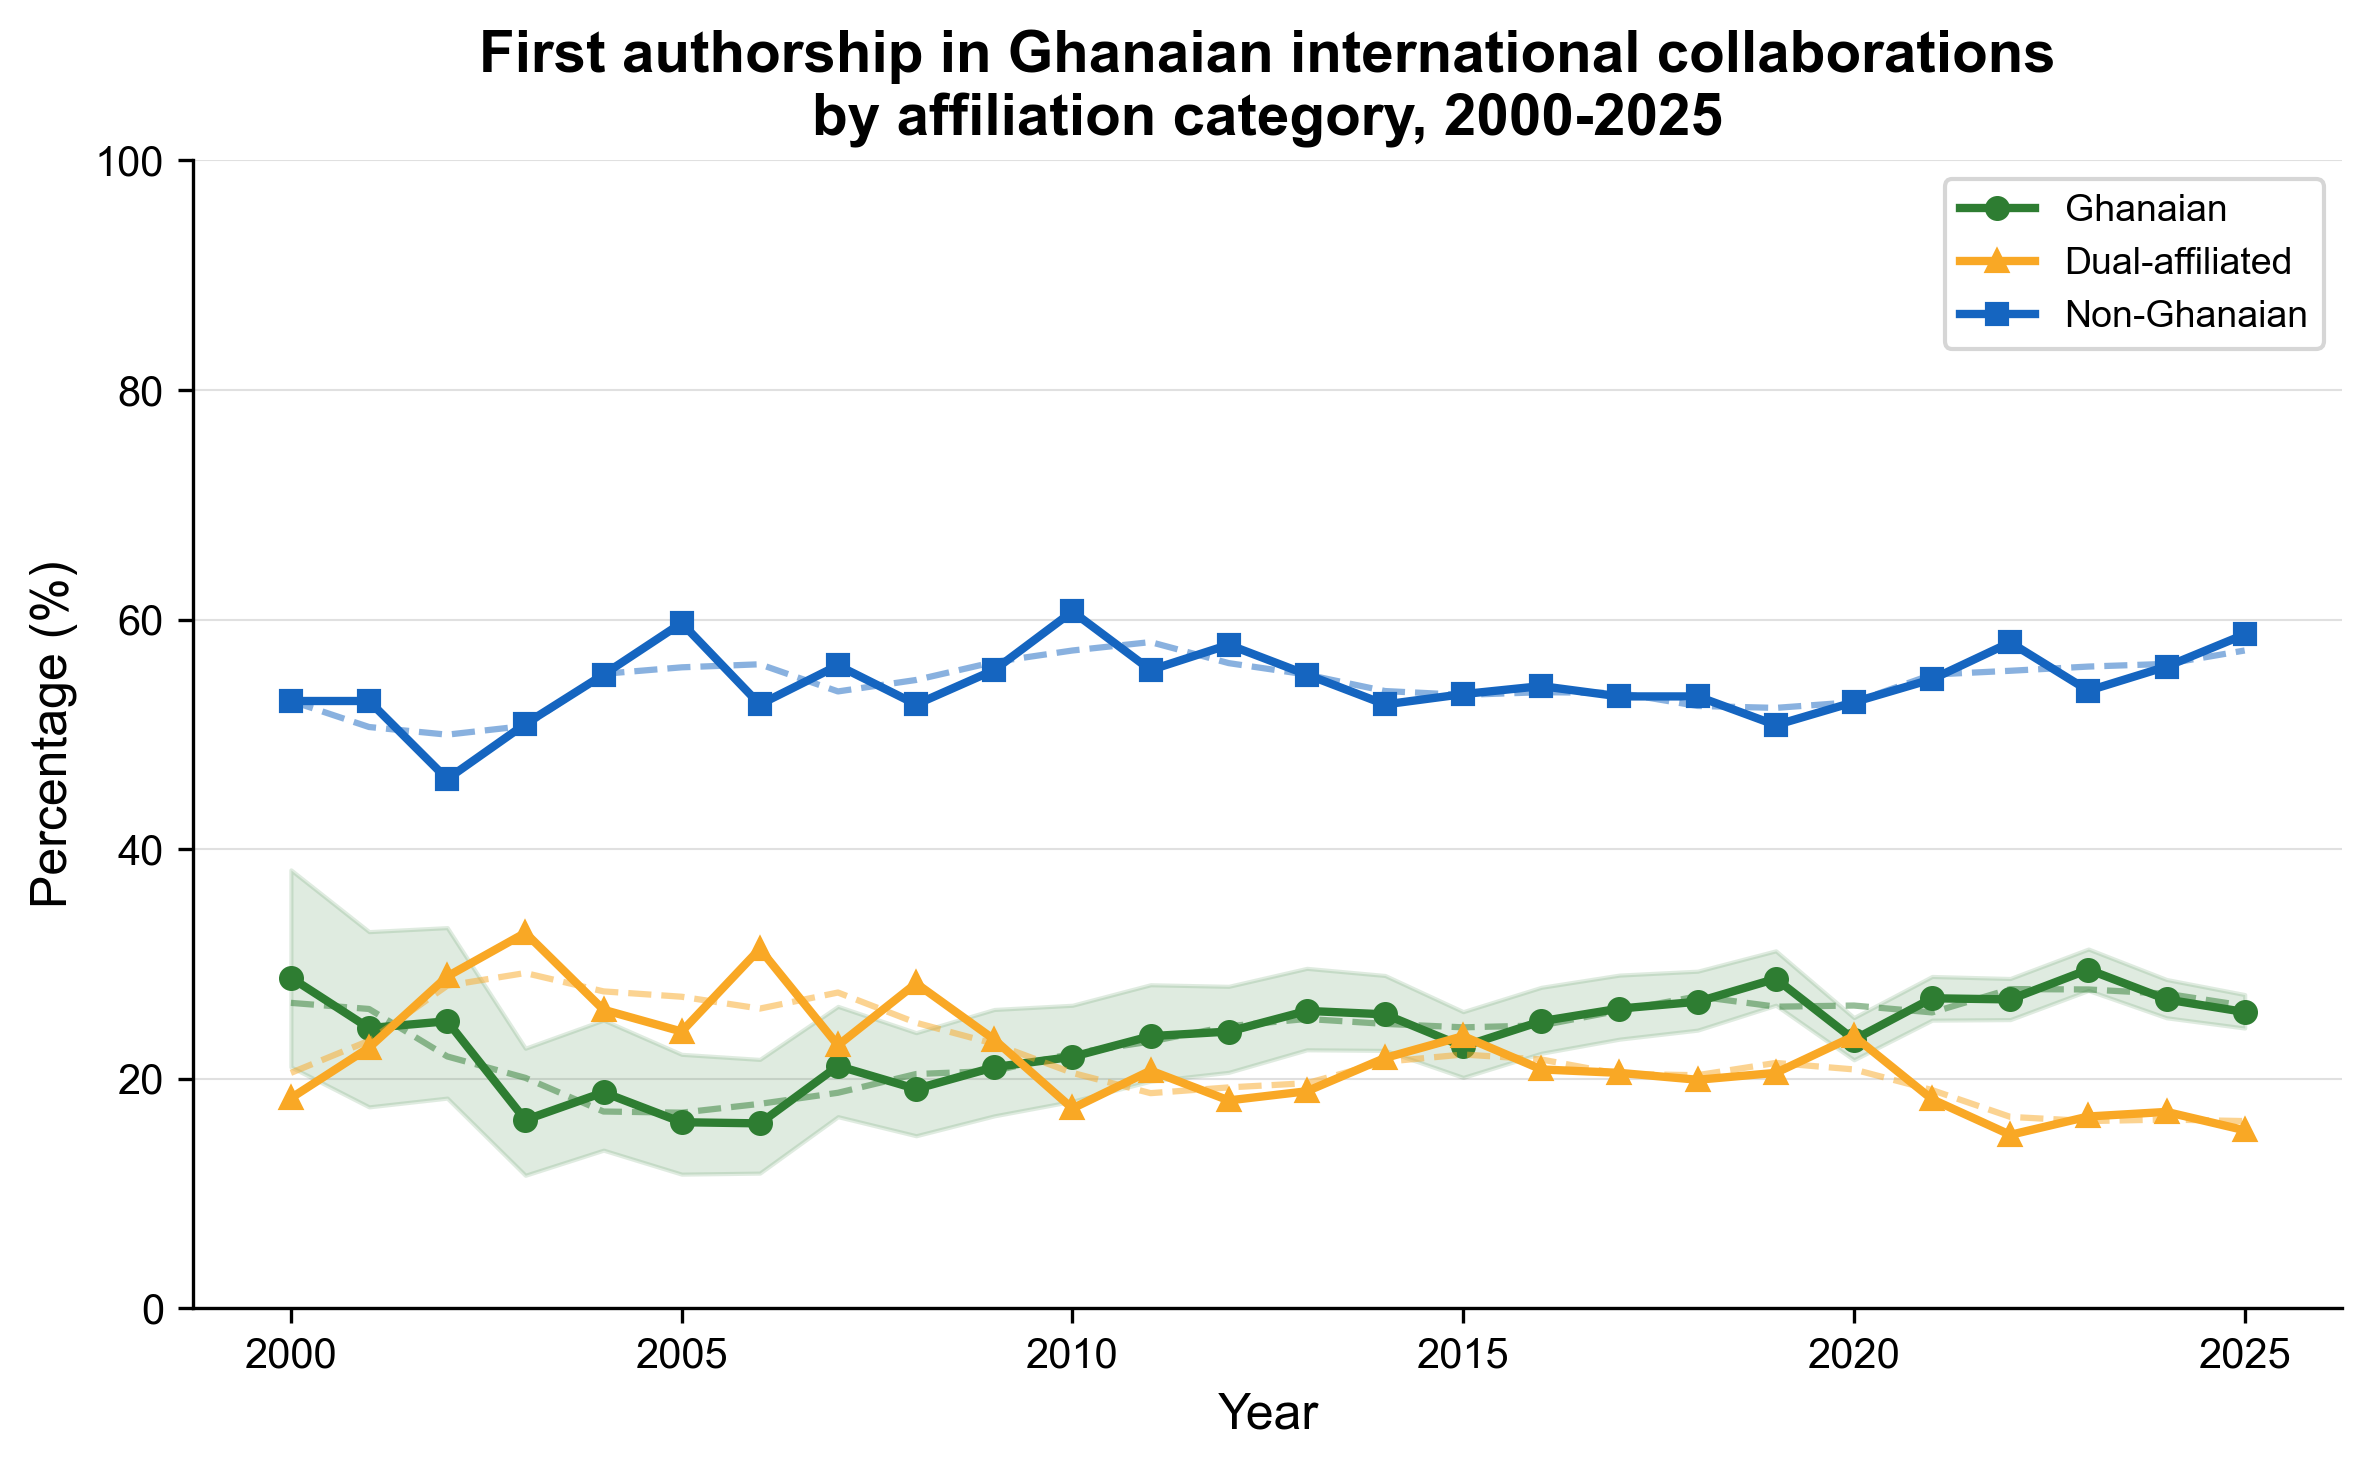
\includegraphics[width=0.92\textwidth]{chart_05_first_author_trend.png}
\caption{Annual proportion of Ghanaian and dual-affiliated first authors, 2000--2025. The fitted trend line shows a declining aggregate proportion (OR = 0.994/year, $p = 0.008$), but multivariate models controlling for team size, partner bloc, and funding reveal a positive adjusted trend (OR = 1.019/year)---a Simpson's paradox driven by the growth of multi-bloc consortia.}
\label{fig:trends}
\end{figure}

However, the multivariate models revealed a striking reversal (Table~\ref{tab:regression}). After adjustment, the year coefficient became positive for first authorship (OR = 1.019, $p < 0.001$) and corresponding authorship (OR = 1.018, $p < 0.001$). This Simpson's paradox arises because multi-bloc collaborations---which show Ghanaian first authorship of only 27.1\%---grew substantially as a proportion of output. The aggregate proportion declined even as the conditional probability of leadership in comparable publications increased. A Ghanaian researcher leading a bilateral study with a UK partner would have higher odds of first authorship in 2020 than in 2005, but the 2020 landscape includes far more consortium papers where local leadership is structurally suppressed.

\subsection{The Bilateral--Consortium Divide}

Decomposition by partnership structure revealed the most important structural finding (Table~\ref{tab:bilateral}). In bilateral partnerships ($n = 16{,}077$; 64.9\%), Ghanaian and dual-affiliated researchers held a majority of first authorships (54.5\%) and corresponding authorships (51.2\%). The aggregate leadership deficit is driven almost entirely by multi-bloc collaborations ($n = 8{,}691$; 35.1\%), where first authorship dropped to 27.1\% and last authorship to 20.9\%. International collaboration, per se, does not disadvantage Ghanaian researchers; rather, the governance structures of large consortia---with centralised analysis units, multiple writing committees, and funder-driven authorship norms---systematically reduce local leadership.

\begin{table}[H]
\centering
\caption{Ghanaian leadership (Ghanaian + Dual-affiliated) by partnership structure}
\label{tab:bilateral}
\begin{tabular}{l c c}
\toprule
\textbf{Position} & \textbf{Bilateral ($N = 16{,}077$)} & \textbf{Multi-bloc ($N = 8{,}691$)} \\
\midrule
First author        & 54.5\% & 27.1\% (95\% CI: 26.2--28.0) \\
Last author         & 40.7\% & 20.9\% \\
Corresponding author & 51.2\% & 23.6\% \\
\bottomrule
\end{tabular}
\end{table}

\subsection{Leadership by Partner Region}

The geographic composition of partnerships significantly shaped Ghanaian leadership (Figure~\ref{fig:bloc}). African (South-South) collaborations yielded the highest rates: 61.2\% (95\% CI: 59.4--63.0) first author, 48.8\% last author, and 60.6\% corresponding author were Ghanaian or dual-affiliated. Western partnerships yielded intermediate rates (54.4\%; 95\% CI: 53.5--55.4), while East Asian (45.1\%; 95\% CI: 42.8--47.4) and South Asian (48.3\%; 95\% CI: 43.7--53.0) partnerships showed lower rates.

Chi-square tests confirmed significant differences between Western and African partnerships at all positions (first: $\chi^2 = 39.48$; last: $\chi^2 = 82.04$; corresponding: $\chi^2 = 80.31$; all $p < 0.001$). The largest statistic for last authorship indicates that the senior leadership gap is most pronounced between North-South and South-South collaborations. Bonferroni-corrected pairwise comparisons confirmed significant differences for first authorship between Western and African ($\chi^2 = 39.48$, $p < 0.001$), Western and East Asian ($\chi^2 = 53.09$, $p < 0.001$), and Western and South Asian partnerships ($\chi^2 = 6.21$, $p = 0.013$).

\begin{figure}[H]
\centering
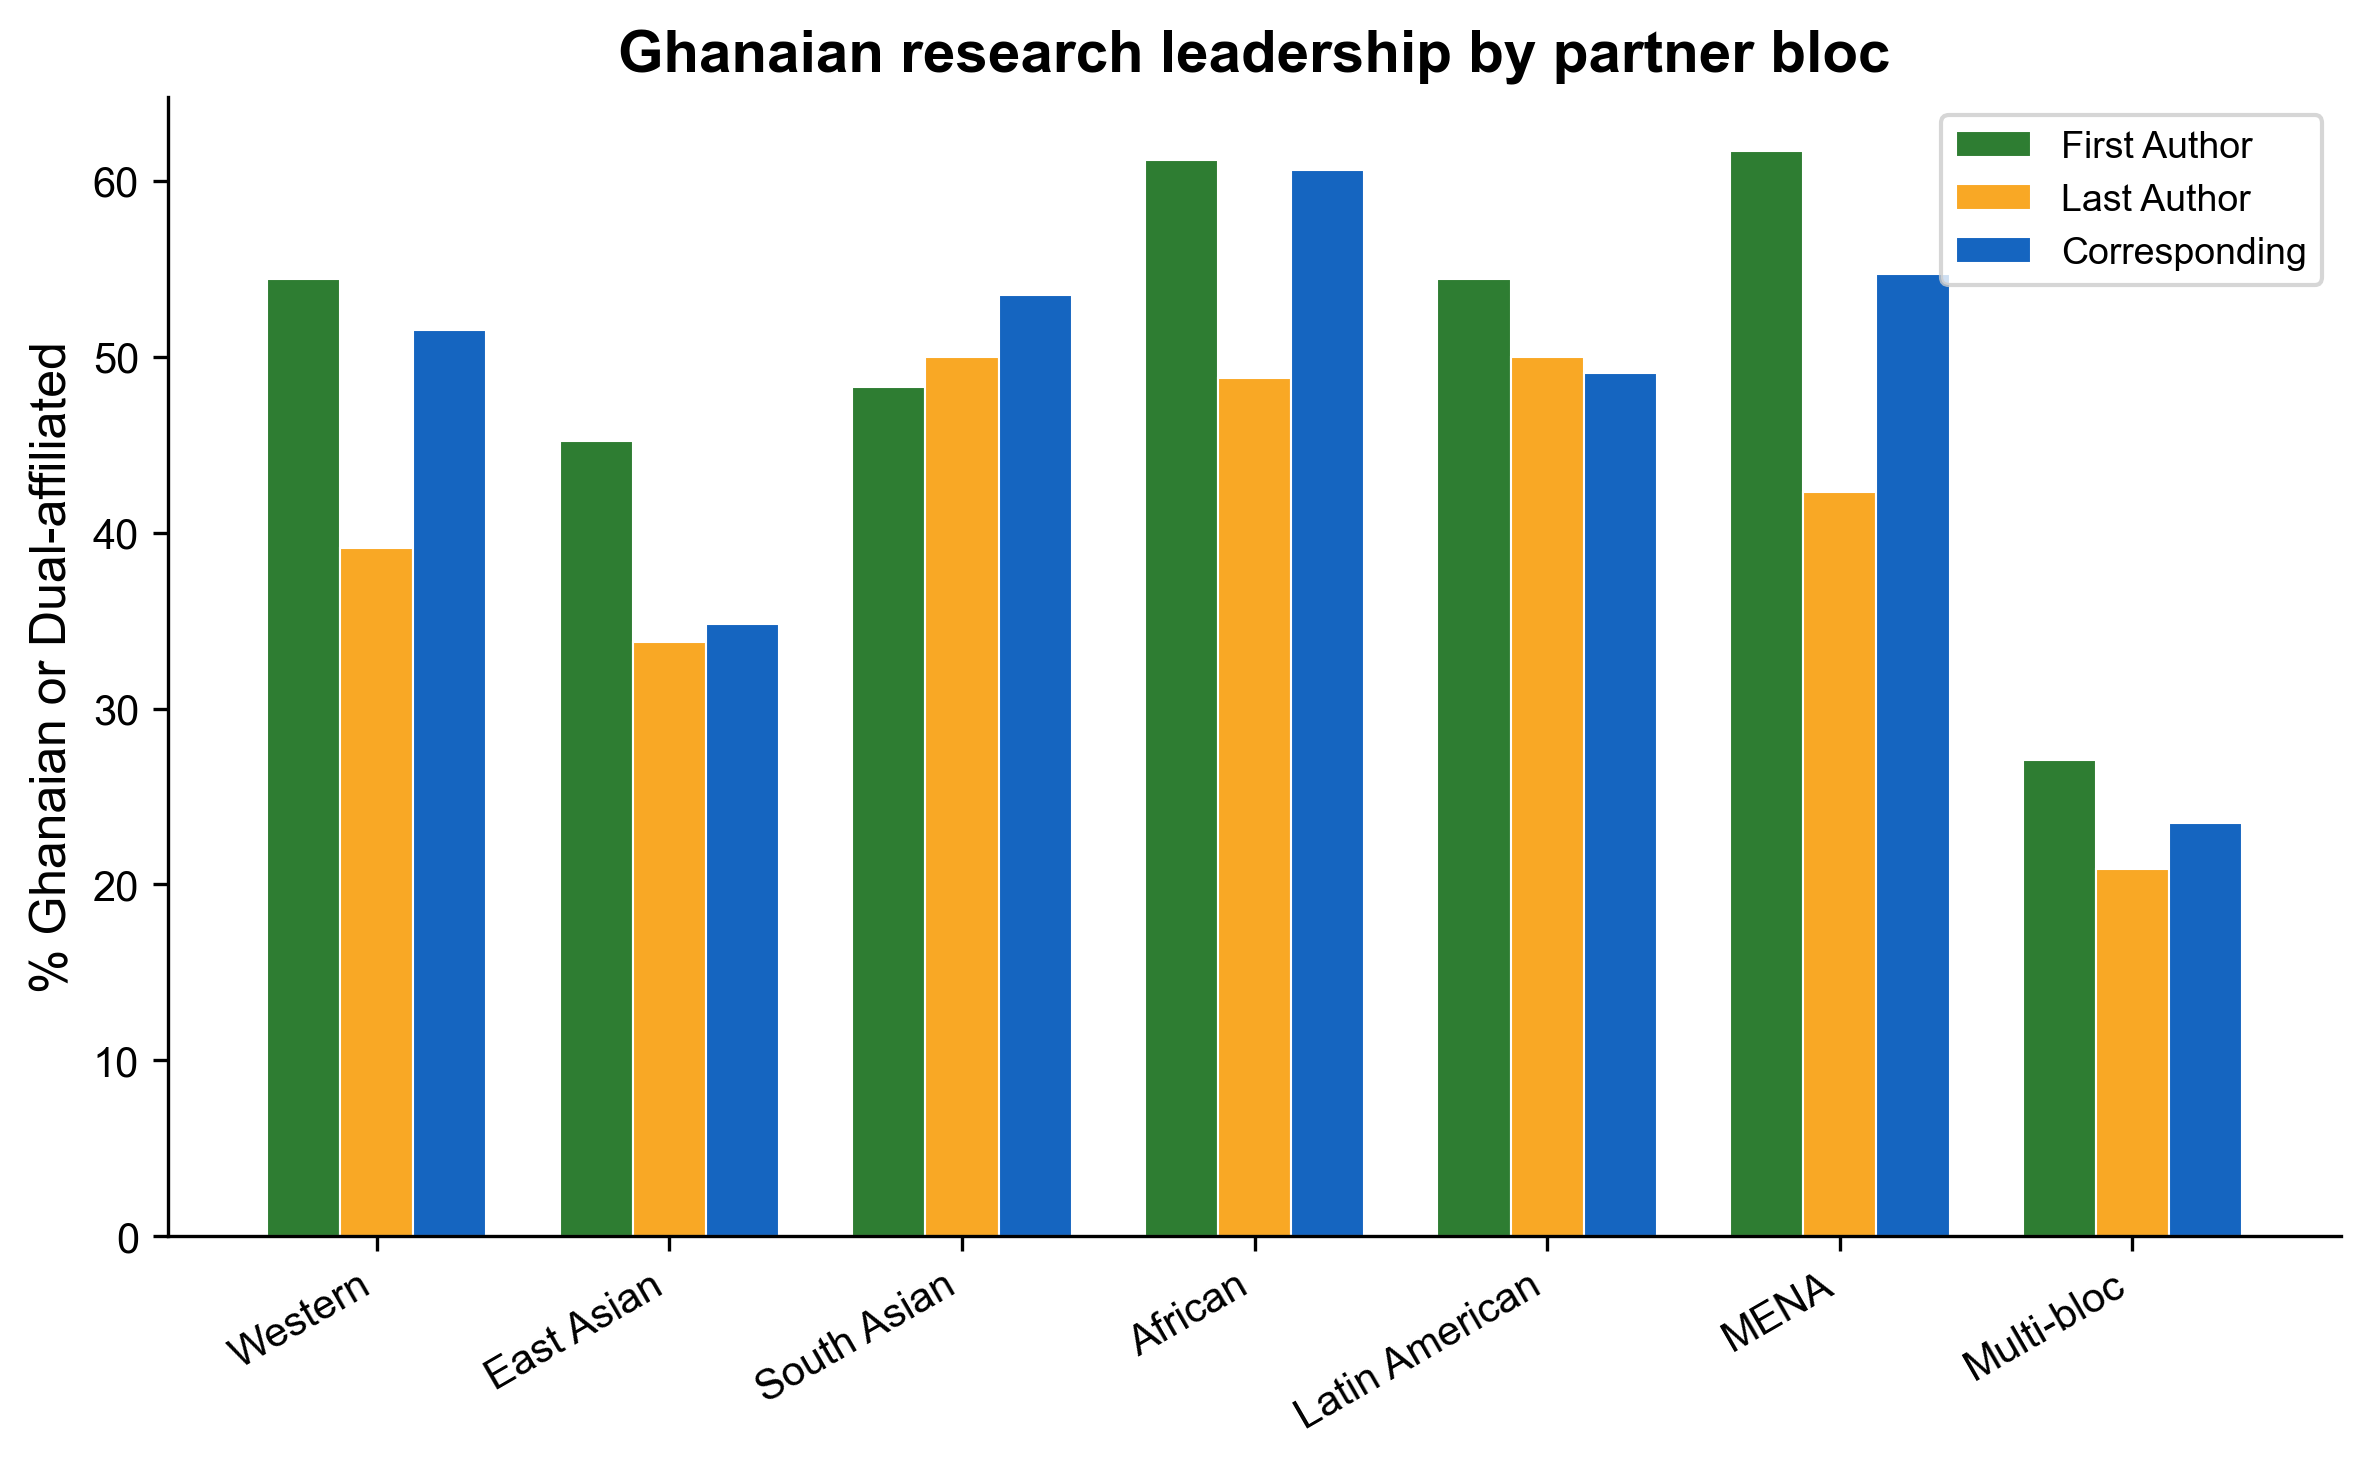
\includegraphics[width=0.92\textwidth]{chart_20_leadership_by_partner_bloc.png}
\caption{Proportion of Ghanaian and dual-affiliated researchers in first, last, and corresponding authorship by partner bloc. Error bars represent 95\% Wilson confidence intervals. African partnerships show the highest equity; multi-bloc collaborations the lowest.}
\label{fig:bloc}
\end{figure}

Country-level analyses with Wilson confidence intervals revealed further variation. China (2,040 collaborations) showed 30.7\% Ghanaian first authorship (95\% CI: 28.8--32.8); India (1,414 collaborations) 23.4\% (95\% CI: 21.3--25.7); South Africa (3,063 collaborations) 37.1\% (95\% CI: 35.4--38.8); and Brazil (514 collaborations) 11.5\% (95\% CI: 9.0--14.5). These findings demonstrate that emerging-power partnerships replicate---and in some cases worsen---the authorship inequities traditionally associated with North-South collaborations.

\subsection{Funding and Leadership}

External funding was a consistent negative predictor across all three positions (Table~\ref{tab:regression}): first author OR = 0.783 (95\% CI: 0.739--0.830), last author OR = 0.667 (95\% CI: 0.627--0.710), and corresponding OR = 0.724 (95\% CI: 0.683--0.767). Chi-square tests comparing Northern-funded, Ghanaian-funded, and unfunded papers confirmed highly significant effects (first: $\chi^2(2) = 634.57$; last: $\chi^2(2) = 488.43$; corresponding: $\chi^2(2) = 1{,}206.93$; all $p < 0.001$). The chi-square for corresponding authorship was nearly double that for first authorship, indicating that funding exerts the strongest control over who serves as the intellectual custodian of the published work.

\subsection{COVID-19 Effects}

Pre-/post-COVID comparisons revealed position-specific shifts (Table~\ref{tab:covid}). Combined Ghanaian + dual-affiliated first authorship \emph{declined} from 46.1\% to 44.0\% ($-2.1$~pp), as the rise in Ghanaian-only authors (24.5\% $\rightarrow$ 26.6\%) was more than offset by a dual-affiliated decline (21.6\% $\rightarrow$ 17.4\%). Last authorship genuinely improved (32.7\% $\rightarrow$ 34.5\%, $+1.8$~pp)---the only position with a net combined gain. Corresponding authorship declined (41.6\% $\rightarrow$ 39.3\%, $-2.3$~pp), driven by a 5.2~pp drop in dual-affiliated corresponding authorship---the single largest category shift in the dataset. Chi-square tests confirmed significance at all positions ($p < 0.001$).

After removing 781 COVID-topic papers, the combined first authorship decline persisted (46.2\% $\rightarrow$ 44.6\%), confirming structural rather than topic-driven change. Using Ghanaian-only rates, the improvement also persisted (24.5\% $\rightarrow$ 27.0\%), indicating genuine domestic capacity growth.

\begin{table}[H]
\centering
\caption{Pre-COVID (2000--2019) vs.\ post-COVID (2020--2025) leadership composition}
\label{tab:covid}
\begin{tabular}{l l r r r}
\toprule
\textbf{Position} & \textbf{Category} & \textbf{Pre-COVID (\%)} & \textbf{Post-COVID (\%)} & \textbf{Change (pp)} \\
\midrule
\multirow{3}{*}{First author} & Ghanaian & 24.5 & 26.6 & $+2.1$ \\
 & Dual-affiliated & 21.6 & 17.4 & $-4.2$ \\
 & \textbf{Combined (GH+Dual)} & \textbf{46.1} & \textbf{44.0} & $\mathbf{-2.1}$ \\
\midrule
\multirow{3}{*}{Last author} & Ghanaian & 19.9 & 23.3 & $+3.4$ \\
 & Dual-affiliated & 12.8 & 11.2 & $-1.6$ \\
 & \textbf{Combined (GH+Dual)} & \textbf{32.7} & \textbf{34.5} & $\mathbf{+1.8}$ \\
\midrule
\multirow{3}{*}{Corresponding} & Ghanaian & 22.6 & 25.5 & $+2.9$ \\
 & Dual-affiliated & 19.0 & 13.8 & $-5.2$ \\
 & \textbf{Combined (GH+Dual)} & \textbf{41.6} & \textbf{39.3} & $\mathbf{-2.3}$ \\
\bottomrule
\multicolumn{5}{l}{\footnotesize $\chi^2$ tests: first $\chi^2(2) = 69.20$; last $\chi^2(2) = 46.89$; corresponding $\chi^2(2) = 149.06$; all $p < 0.001$.} \\
\end{tabular}
\end{table}

\begin{figure}[H]
\centering
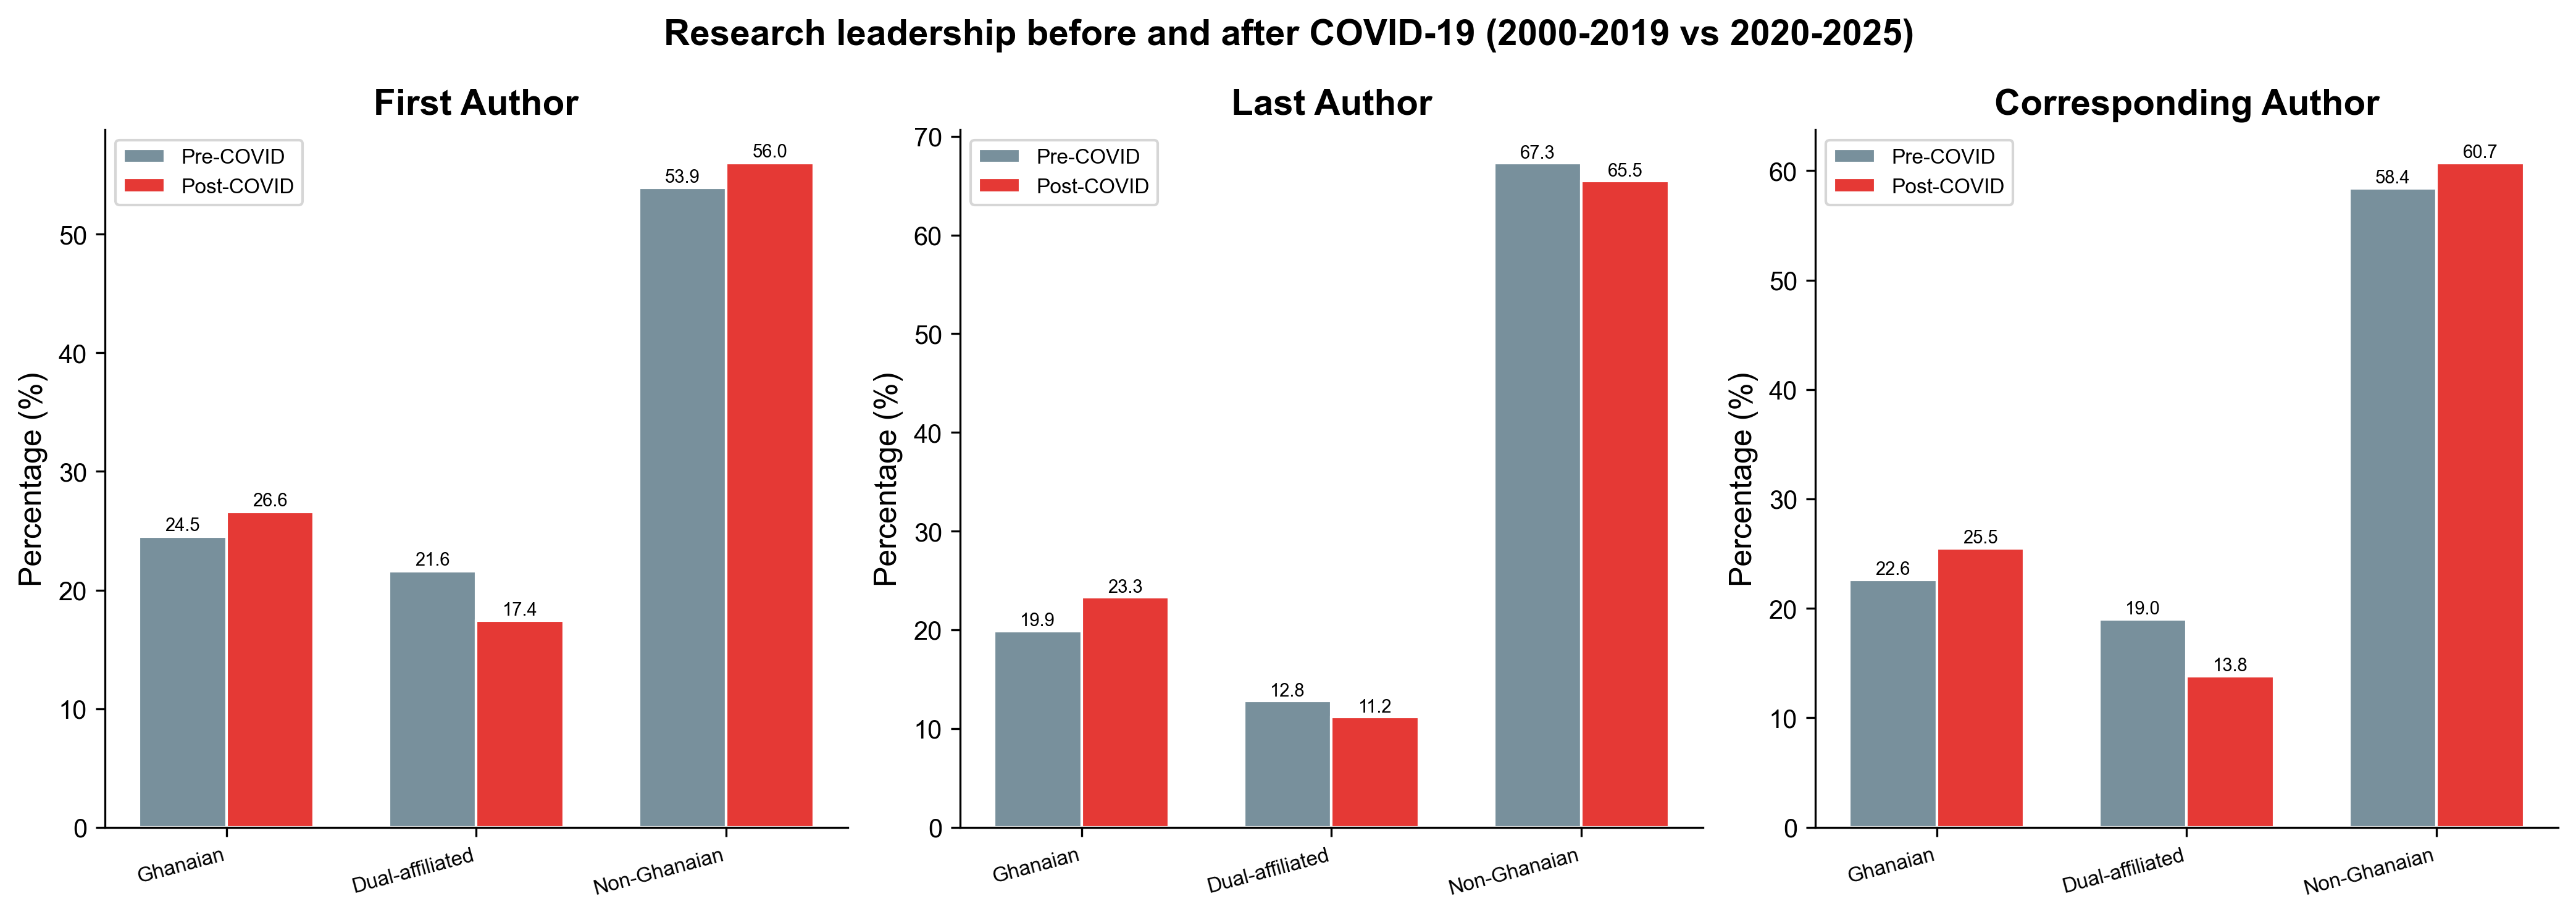
\includegraphics[width=0.92\textwidth]{chart_18_pre_post_covid_comparison.png}
\caption{Pre-COVID (2000--2019) vs.\ post-COVID (2020--2025) leadership composition by affiliation category. Combined Ghanaian + dual-affiliated first and corresponding authorship both declined; only last authorship showed a net combined improvement ($+1.8$~pp).}
\label{fig:covid}
\end{figure}

\subsection{Multivariate Logistic Regression}

Three logistic regression models identified structural predictors of Ghanaian leadership (Table~\ref{tab:regression}). Across all models, the number of partner countries was the single strongest negative predictor (ORs: 0.690--0.749), followed by funding status (ORs: 0.667--0.783). Open access publication was consistently positive (ORs: 1.213--1.369).

The pseudo-$R^2$ values (0.089--0.100) are modest but characteristic of bibliometric regressions, where authorship decisions depend on unmeasurable factors---personal relationships, laboratory hierarchies, career stage, and negotiation dynamics. The models identify structural factors that systematically shift the probability of Ghanaian leadership while acknowledging substantial unexplained variance.

The COVID era coefficient differed between models: negative for first authorship (OR = 0.899, $p = 0.022$) but positive for last authorship (OR = 1.196, $p < 0.001$). These are not contradictory: the positive year trend (OR = 1.019/year) accumulates over 20 years, so by 2020 the cumulative effect is strongly positive. The COVID binary captures the discrete residual shift beyond the year trend---slightly negative for first authorship, genuinely positive for last authorship, and not significant for corresponding authorship.

Field effects were position-dependent. Engineering was the strongest positive predictor across all models (ORs: 1.260--2.036), with the last authorship effect (OR = 2.036) indicating Ghanaian engineers were approximately twice as likely to occupy senior positions. Health Sciences (incorporating Medicine, Nursing, and Health Professions) was a significant positive predictor for last authorship (OR = 1.496) and corresponding authorship (OR = 1.188), suggesting Ghanaian senior researchers have a structural advantage in applied clinical disciplines where local knowledge is indispensable.

\begin{table}[H]
\centering
\caption{Multivariate logistic regression models for Ghanaian research leadership}
\label{tab:regression}
\small
\begin{tabular}{l c c c}
\toprule
 & \textbf{Model 1: First} & \textbf{Model 2: Last} & \textbf{Model 3: Corresponding} \\
\textbf{Predictor} & OR (95\% CI) & OR (95\% CI) & OR (95\% CI) \\
\midrule
Year (centred) & 1.019 (1.011--1.027)*** & --- & 1.018 (1.010--1.026)*** \\
Country count & 0.689 (0.667--0.712)*** & 0.707 (0.681--0.734)*** & 0.749 (0.728--0.771)*** \\
Author count & 0.978 (0.973--0.984)*** & 0.961 (0.954--0.968)*** & 0.980 (0.974--0.985)*** \\
Funding (yes) & 0.784 (0.740--0.831)*** & 0.664 (0.625--0.707)*** & 0.724 (0.684--0.767)*** \\
Open access (yes) & 1.211 (1.136--1.291)*** & 1.346 (1.259--1.440)*** & 1.368 (1.283--1.459)*** \\
COVID era & 0.899 (0.821--0.985)* & 1.198 (1.089--1.318)*** & --- \\
\midrule
\multicolumn{4}{l}{\textit{Partner bloc (ref: African)}} \\
\quad Western & 0.853 (0.781--0.933)*** & 0.777 (0.711--0.848)*** & 0.819 (0.750--0.895)*** \\
\quad East Asian & 0.530 (0.468--0.601)*** & 0.594 (0.523--0.676)*** & 0.435 (0.383--0.494)*** \\
\quad South Asian & 0.519 (0.423--0.636)*** & --- & --- \\
\quad Multi-bloc & 0.645 (0.578--0.719)*** & 0.755 (0.674--0.845)*** & 0.619 (0.556--0.688)*** \\
\midrule
\multicolumn{4}{l}{\textit{Field (ref: Biochemistry/Genetics)}} \\
\quad Engineering & 1.261 (1.121--1.419)*** & 2.032 (1.785--2.313)*** & 1.590 (1.412--1.790)*** \\
\quad Health Sciences & --- & 1.496 (1.332--1.681)*** & 1.188 (1.071--1.318)** \\
\midrule
AIC & 30{,}693.3 & 28{,}723.1 & 31{,}003.5 \\
Pseudo-$R^2$ & 0.100 & 0.089 & 0.090 \\
\bottomrule
\multicolumn{4}{l}{\footnotesize $*\,p < 0.05$;\;\; $**\,p < 0.01$;\;\; $***\,p < 0.001$. ``---'' indicates predictor was not significant ($p > 0.05$).} \\
\multicolumn{4}{l}{\footnotesize Only significant predictors shown. VIF for year and COVID era: 2.80.} \\
\end{tabular}
\end{table}

\begin{figure}[H]
\centering
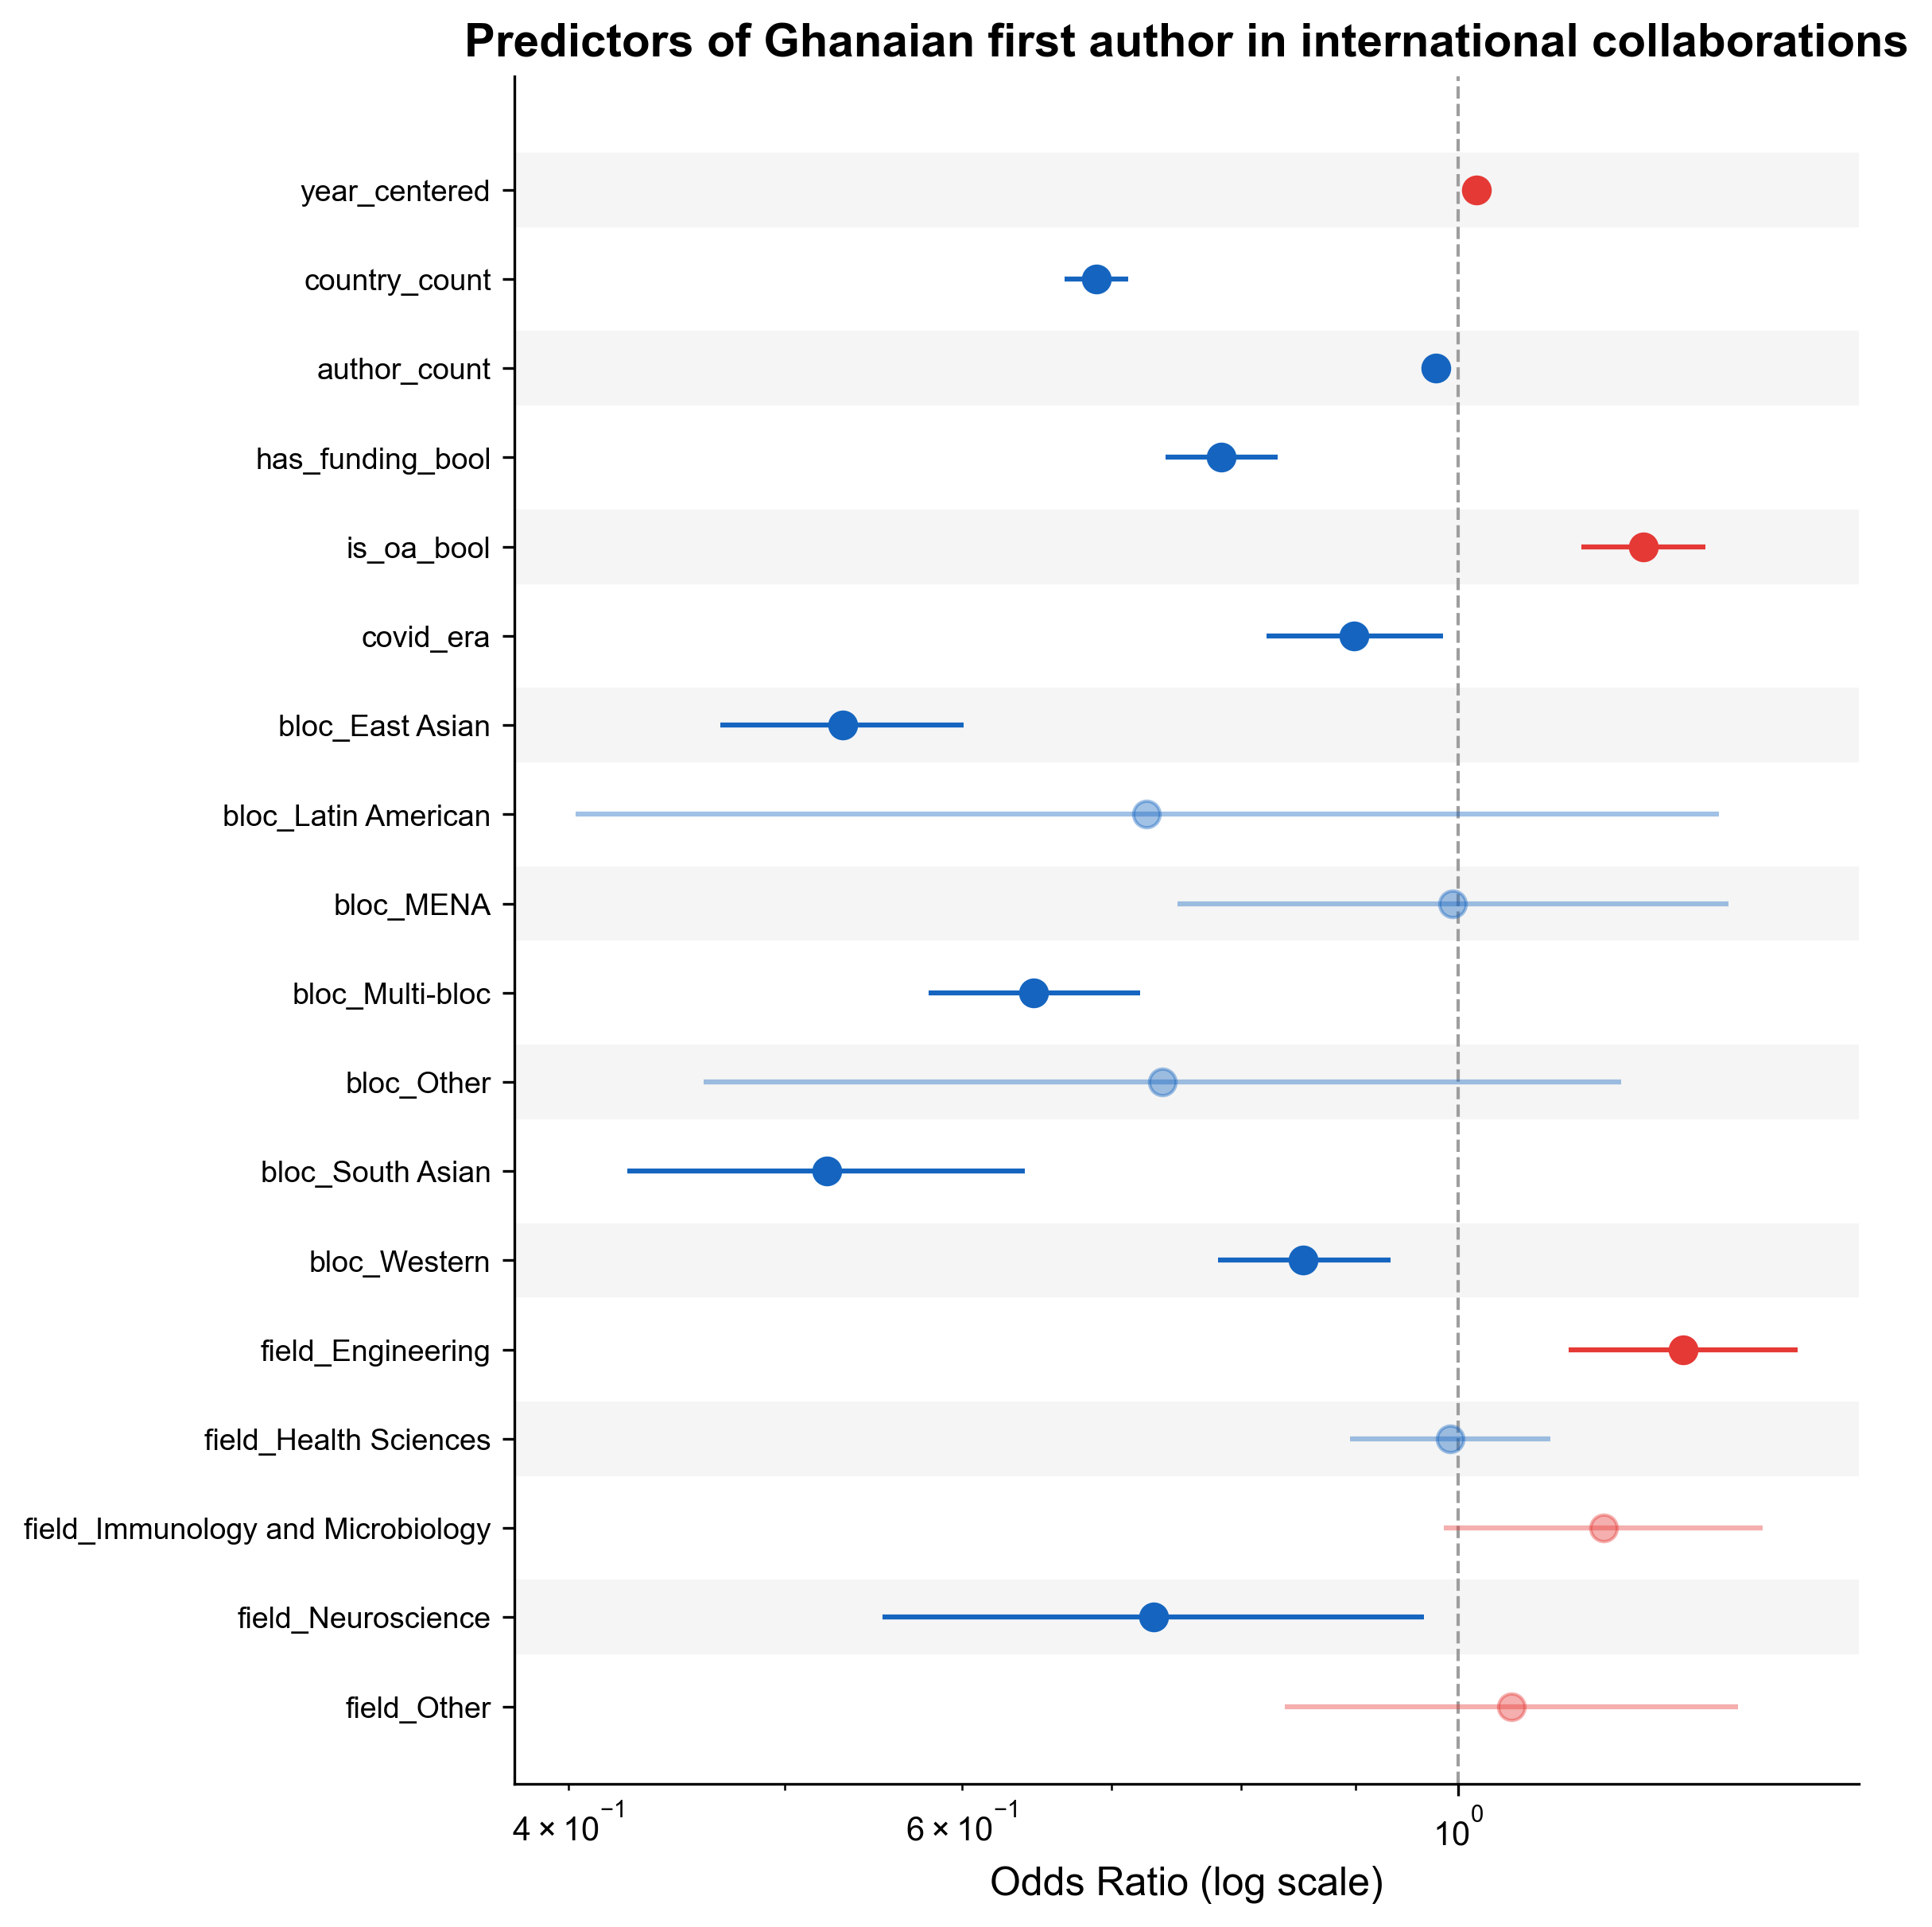
\includegraphics[width=0.92\textwidth]{chart_13_forest_plot_model1.png}
\caption{Forest plot of odds ratios from the first authorship logistic regression model (Model~1). Country count is the strongest negative predictor (OR = 0.690); Engineering the strongest positive field effect (OR = 1.259). Reference categories: African bloc, Biochemistry/Genetics field.}
\label{fig:forest}
\end{figure}

\subsection{Citation Impact}

Among 22,684 works with FWCI data, papers led by non-Ghanaian first authors showed significantly higher citation impact (median FWCI = 1.27, IQR: 0.20--3.42) than Ghanaian-led (0.86, IQR: 0.00--2.39) or dual-affiliated-led papers (0.80, IQR: 0.00--2.35). Mann-Whitney $U$ tests confirmed these differences (Ghanaian vs.\ non-Ghanaian: $U = 32{,}400{,}962$, $p < 0.001$; dual-affiliated vs.\ non-Ghanaian: $U = 23{,}255{,}833$, $p < 0.001$). The counterintuitively lower FWCI for dual-affiliated papers may reflect selection into smaller bilateral studies while higher-impact work is credited to non-Ghanaian affiliations, or the inclusion of administrative appointments with limited research engagement.

Among FWCI-available works, 31.3\% of non-Ghanaian-led papers fell in the top 10\% of cited publications (3,938/12,585), compared to 22.6\% for both Ghanaian-led (1,328/5,866) and dual-affiliated-led papers (957/4,233). This gap likely reflects structural advantages---journal prestige networks, topic selection, institutional reputation---rather than inherent quality differences.

\begin{figure}[H]
\centering
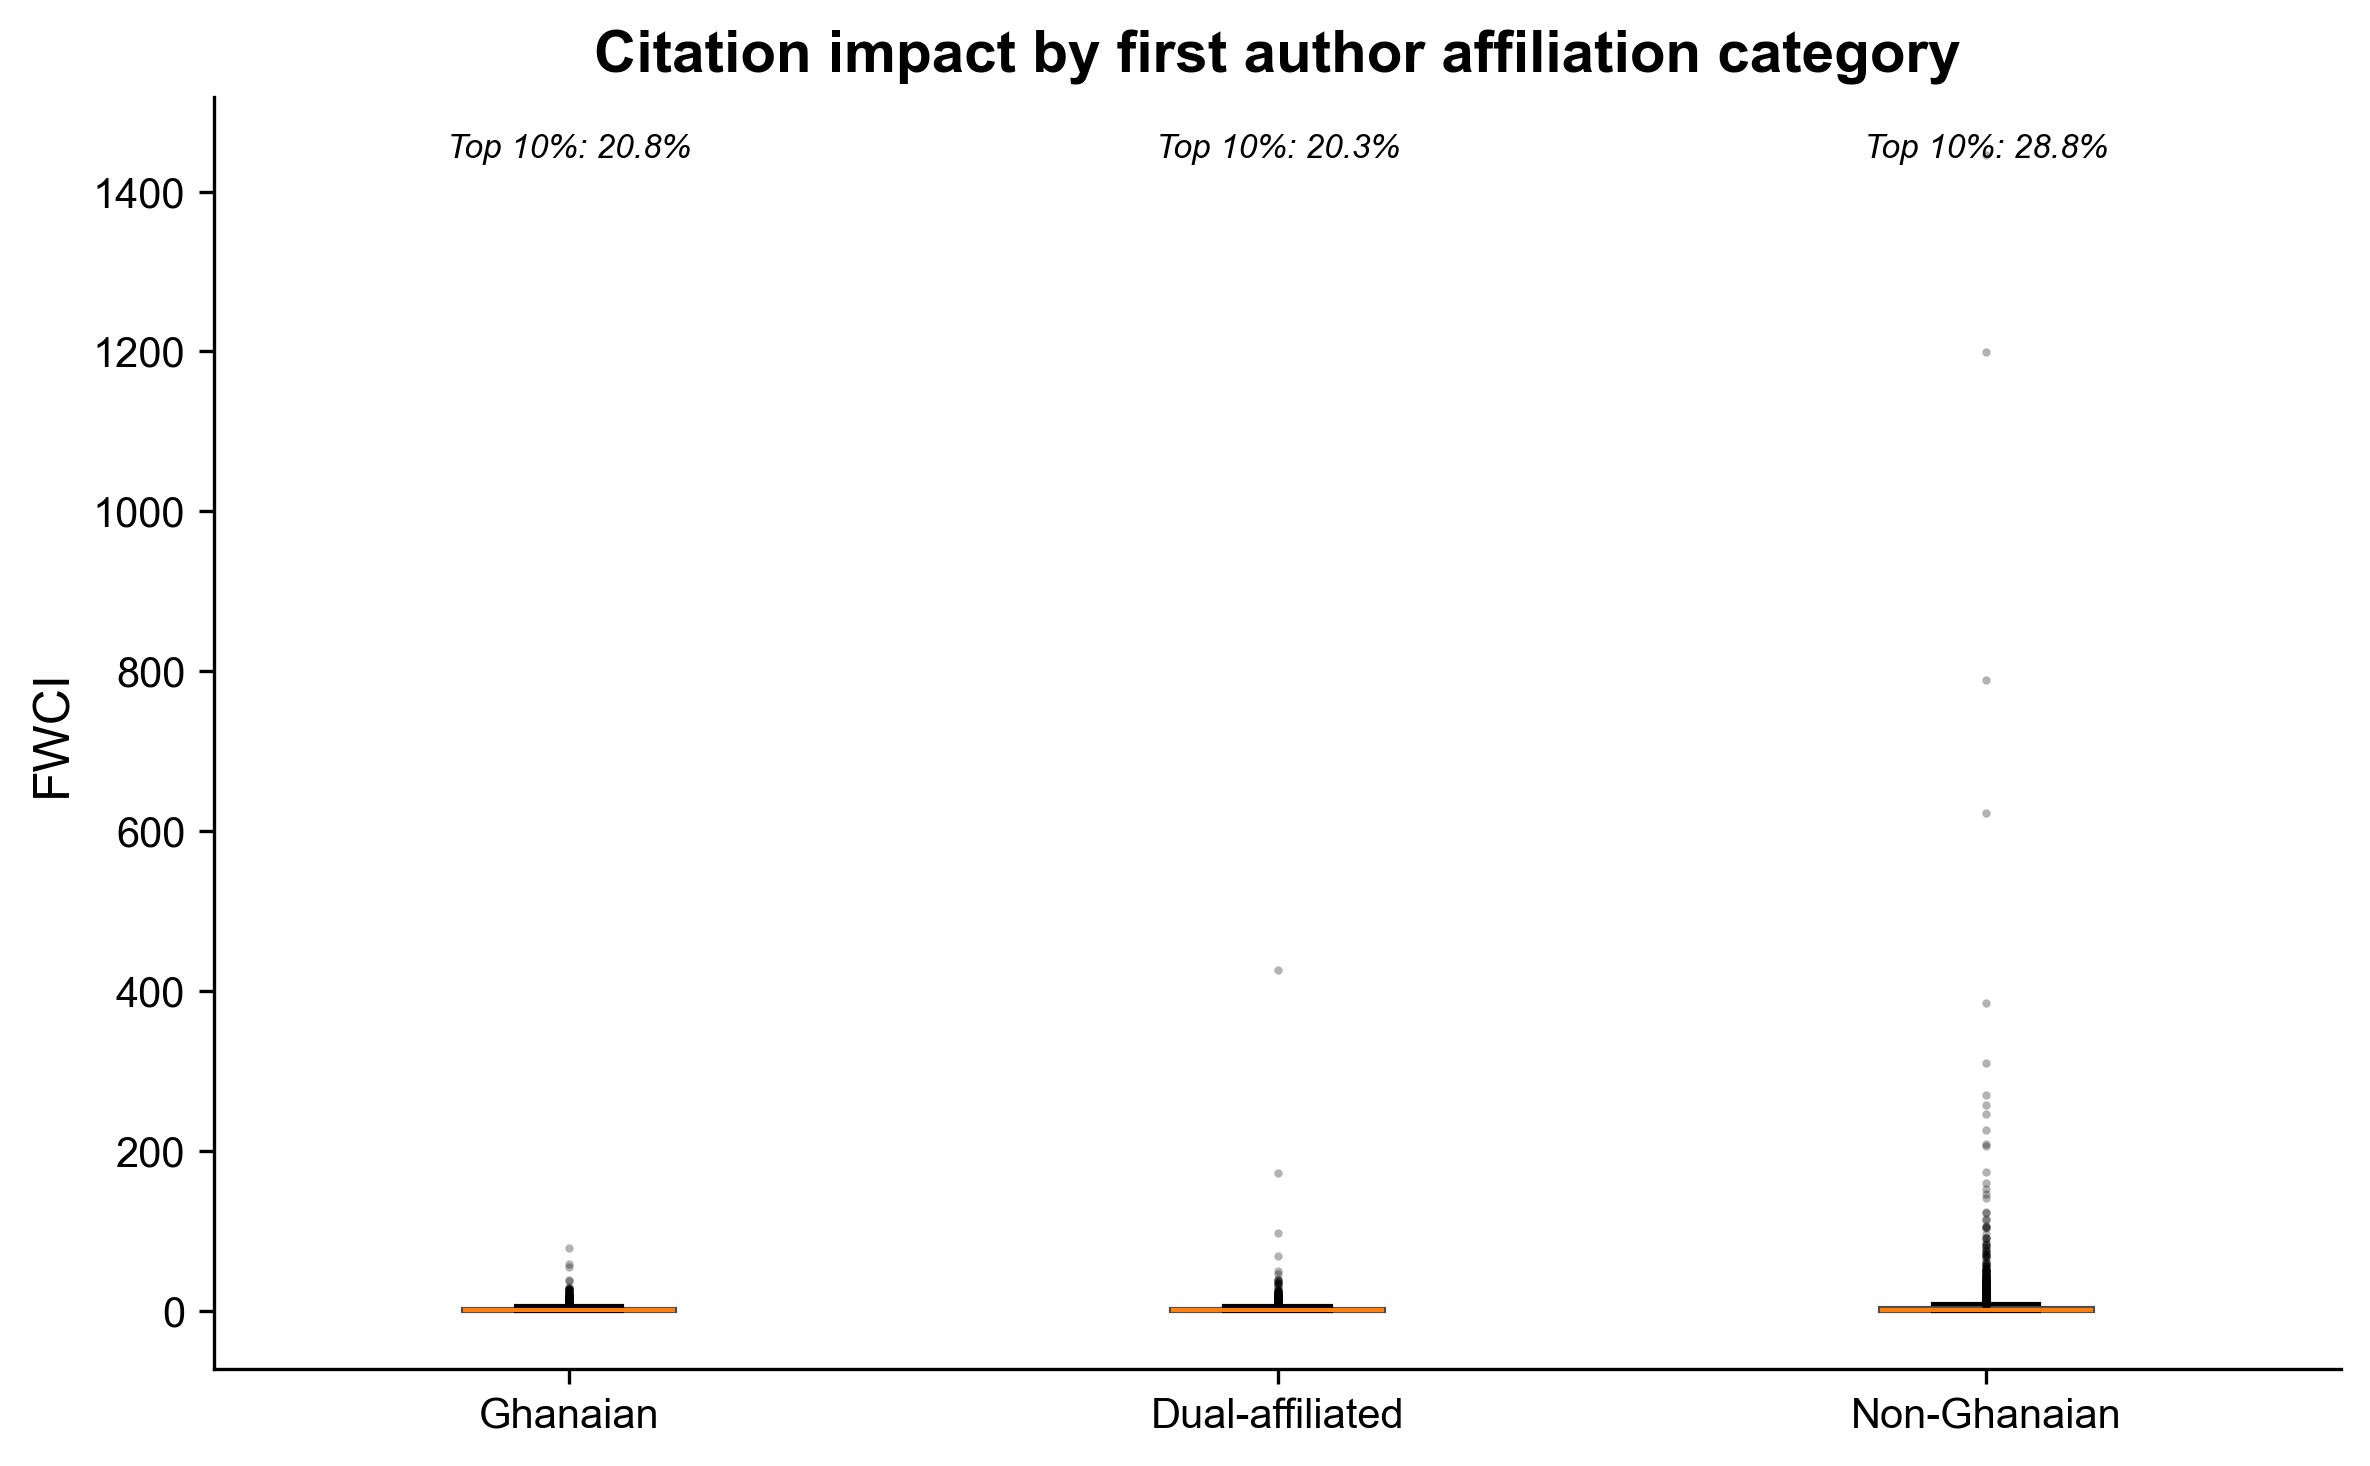
\includegraphics[width=0.88\textwidth]{chart_12_citations_by_leader.png}
\caption{Field-Weighted Citation Impact (FWCI) distribution by first author affiliation category ($n = 22{,}684$ works with FWCI data). Non-Ghanaian-led papers show significantly higher median FWCI (1.27) than Ghanaian-led (0.86) or dual-affiliated-led papers (0.80; Mann-Whitney $U$, $p < 0.001$).}
\label{fig:citations}
\end{figure}

\subsection{Institutional Variation}

Among the top five Ghanaian institutions, leadership rates varied substantially (Table~\ref{tab:institutions}). The University of Cape Coast and the University of Health and Allied Sciences showed the highest first authorship rates (55.4\% each), while the University of Ghana---despite the highest absolute volume (7,709 works)---showed the lowest rates (44.5\% first, 33.0\% last). This mirrors the bilateral-consortium divide: institutions embedded in large consortium networks show lower leadership rates.

\begin{table}[H]
\centering
\caption{Research leadership rates at top Ghanaian institutions}
\label{tab:institutions}
\small
\begin{tabular}{l r r r r}
\toprule
\textbf{Institution} & \textbf{Works} & \textbf{First (\%)} & \textbf{Last (\%)} & \textbf{Corr.\ (\%)} \\
\midrule
University of Cape Coast & 2,325 & 55.4 & 37.3 & 49.2 \\
Univ.\ of Health \& Allied Sciences & 2,230 & 55.4 & 39.2 & 50.7 \\
KNUST & 5,692 & 52.3 & 38.2 & 46.4 \\
Noguchi Memorial Institute & 1,963 & 49.6 & 34.4 & 38.7 \\
University of Ghana & 7,709 & 44.5 & 33.0 & 38.7 \\
\bottomrule
\multicolumn{5}{l}{\footnotesize Ghanaian + Dual-affiliated proportions. KNUST = Kwame Nkrumah Univ.\ of Science and Technology.} \\
\end{tabular}
\end{table}

\subsection{Sensitivity Analyses}

All six sensitivity analyses confirmed the robustness of primary findings. Reclassifying dual-affiliated authors as Ghanaian yielded 44.9\% first authorship; reclassifying as non-Ghanaian yielded 25.8\%---core conclusions unchanged in either scenario. Restricting to journal articles only ($n = 19{,}788$, 79.9\%) produced nearly identical proportions (Ghanaian first author: 26.5\%). All 26 study years met $\geq$50\% corresponding author coverage. No works had truncated author lists; excluding 337 works with $>$50 authors yielded 26.1\% Ghanaian first authorship. After removing 781 COVID-topic papers, the combined (GH+Dual) first authorship decline persisted (46.2\% $\rightarrow$ 44.6\%), and Bonferroni-corrected bloc comparisons remained significant.

% ============================================================
\section{Discussion}
% ============================================================

This study of 24,768 international collaborative publications reveals a persistent but structurally nuanced leadership deficit for Ghanaian researchers in biomedical science and engineering. Three findings merit particular attention.

\subsection{The Consortium Problem}

The bilateral-consortium decomposition reframes the equity narrative. In bilateral partnerships---which represent nearly two-thirds of all collaborations---Ghanaian and dual-affiliated researchers hold a majority of first authorships (54.5\%) and corresponding authorships (51.2\%). The aggregate deficit is driven almost entirely by multi-bloc collaborations, where first authorship drops to 27.1\%. This distinction has direct policy implications: the equity challenge lies not in bilateral partnership per se but in the governance structures of large consortia. As consortium-based research has grown, it has progressively diluted aggregate Ghanaian leadership---producing the Simpson's paradox identified in the temporal analysis, where raw trends decline but adjusted trends improve.

\subsection{The Funding-Authorship Nexus}

The consistent negative association between external funding and Ghanaian leadership (ORs: 0.667--0.783) across all three positions, with the strongest effect on corresponding authorship ($\chi^2 = 1{,}206.93$), provides quantitative evidence for the ``he who pays the piper'' hypothesis. The disproportionate effect on corresponding authorship is particularly consequential: this role controls the manuscript during peer review, determines who receives reprint requests, and shapes the long-term intellectual ownership of the work. When funders' institutional nominees serve as corresponding authors, the career benefits of publication accrue primarily to the non-Ghanaian partner.

\subsection{The Corresponding Author Decline}

The monotonic decline in corresponding authorship ($\tau = -0.320$, $p = 0.023$, Sen's slope $= -0.15$~pp/year) is the most concerning temporal finding. While first and last authorship show no significant trend---and multivariate models suggest genuine improvement after adjustment---corresponding authorship is eroding. This decline is occurring even as Ghanaian-only authorship rises, driven by the sharp decline in dual-affiliated corresponding authorship (from 19.0\% to 13.8\% in the COVID transition). The interpretation is cautioned by the finding that 80.1\% of corresponding authors are also first authors, suggesting potential imputation in the source data. However, the distinct patterns observed---the steeper temporal decline and larger funding chi-square relative to first authorship---suggest the corresponding author variable captures meaningful signal beyond mere first-author duplication.

\subsection{Emerging-Power Partnerships}

The finding that collaborations with China (30.7\% Ghanaian first authorship), India (23.4\%), and Brazil (11.5\%) show authorship inequities comparable to or worse than traditional North-South partnerships challenges the assumption that South-South collaboration inherently promotes equity. South Africa (37.1\%)---while better than Asian partners---also falls below the African bloc average, reflecting its position as a regional research power. These findings suggest that research leadership equity is driven less by the Global North/South distinction than by the relative power and institutional capacity of research partners.

\subsection{Limitations}

Several limitations should be considered. First, ``Ghanaian'' is defined by institutional affiliation, not nationality, potentially inflating Ghanaian leadership estimates through expatriate researchers at Ghanaian institutions. Second, the 80.1\% overlap between first and corresponding authorship---likely reflecting OpenAlex imputation---means the corresponding authorship analysis should be interpreted with caution. Third, pseudo-$R^2$ values of 0.089--0.100 indicate that substantial variance in authorship decisions remains unexplained by the measured predictors. Fourth, the study examines biomedical science and engineering; findings may not generalise to other disciplines. Fifth, FWCI coverage of 91.6\%, while high, means citation analyses exclude 8.4\% of works.

\end{document}
